\section{Discusión}

\subsection{Datos a emplear}
Tras comparar los resultados de los tres algoritmos anteriores. Vemos que la tabla final que deberemos usar para el analisis se obtiene usando el tercer metodo, donde no perdemos ninguna proteina virica y unicamente perdemos 4 de las humanas. 
Ya que usando el metodo de biomaRt perdemos 225 genes humanos, perdemos tambien 4 genes viricos pertenecientes al Covid. Y hemos comprobado que usando bitR solo obteniamos 18 de las 332 proteinas humanas y además unicamente dos de las proteinas covid. 

\subsection{Grafo conexo}
Despues de todos los intentos por obtener un grafo conexo, mencionados en el apartado de resultados. Hemos conseguido obtener el grafo conexo, puede que no sea el grafo optimo ni contenga todas las rutas, debido a los diferentes problemas vistos, pero hemos conseguido unir mediante rutas de proteinas humanas, las proteinas del Covid. 
Hemos podido comprobar que el grafo del proteoma total formaba una unica componente conexa, por tanto todas las proteinas se encuentran en el mismo lugar, y pueden usarse las funciones de igraph para conseguir las rutas. 
Tambien se podria haber utilizado las matrices de adyacencia para obtener rutas, tal y como se vio en clase de teoria, pero preferimos haber optado por el metodo del uso de funciones del paquete igraph. La funcion empleada para ver si el grafo obtenido es conexo es components, donde su parametro no indica el numero de componentes, y su parametro csize indica el numero de vertices diferentes. 
Por tanto, obtenemos una red formada por 2888 nodos, 9333 enlaces entre ellos y una unica compoente conexa. De la cual podremos analizar su modularidad y analisis funcional.

\subsection{Comparacion entre la red obtenida y la red humana}
Vistos los resultados de la comparación podremos comentar lo siguiente:
- Vemos que la red de proteoma humana es más densa, por tanto, contiene muchas más conexiones entre nodos que la nueva creada.
- Observamos que la red del porteoma humana tiene caminos mas cortos entre si que la red obtenida, consiguiendo asi una red menos compacta.
- Aqui observamos una de las propiedades de las redes reales donde vemos que tenemos unos pocos nodos de alto grado y muchos nodos de grado mas bajo. 
- Una característica destacable es que en la red humana los nodos con el mismo grado tiende a undirse entres si, pero en nuestra red obtenida la asortatividad es muy baja.
- La distribución de grado es más o menos similar en ambas, y no siguen una distribucion binomial que corresponde a grafo aleatorios. Sino que la frecuencia va aumentando con el grado, para que asi se puedan ir formando los denominados hubs.

\subsection{Centralidad obtenida}
Tras realizar un breve an\'alisis de la centralidad de nuestro modelo usado(hay que recordar que estamos usando un subgrafo que forma una sola componente conexa, porque todo el grafo entero como componente conexa tiene un costo computacional demasiado elevado), hemos obtenido resultados que no eran del todo esperados.\newline
Recapitulando, los valores obtenidos se han normalizado mediante la funci\'on \textbf{closeness} que obtiene la centralidad, es decir, todos los valores de centralidad est\'an comprendidos entre 0 y 1. En primer lugar, hemos obtenido una media de centralidad de 0.287, n\'umero que puede ser considerado muy bajo, dado que podr\'ia llegar hasta 1. Esto quiere decir que probablemente gran parte de nuestros nodos del subgrafo carezcan de importancia dentro de este seg\'un su posici\'on relativa en el subgrafo. Tambi\'en se podr\'ia interpretar como que hay bastantes nodos distanciados del resto de nodos en la red, por lo que la componente conexa que tenemos podr\'ia estar muy dispersa.\newline
Por un lado, no tenemos ning\'un nodo con una centralidad menor de 0.1, sin embargo, la mayor\'ia de los nodos(1990) tienen una centralidad comprendida entre 0.1 y 0.3. Esto nos ayuda a reafirmar que la mayor\'ia de los nodos de la red poseen una centralidad baja. Teniendo en cuenta que estamos midiendo la centralidad con la cercan\'ia, y sabiendo que la centralidad de cercan\'ia de un nodo se calcula como $1/(\Sigma(d(i,j)), i != j)$, tenemos que cuanto mayor sean las distancias de un nodo al resto de nodos, menor centralidad tendr\'a. Dicho de otro modo, la mayor\'ia de los nodos poseen una distancia al resto de nodos bastante elevada.\newline
Por otro lado, aunque hay unos cuantos nodos(898) con un valor de centralidad de entre 0.3 y 0.5, no hay ninguno cuyo valor de centralidad sea mayor que 0.5, lo que nos quiere decir que no hay ning\'un nodo en nuestro subgrafo que pueda ser considerado central o importante. Esto puede deberse, o bien a que el subgrafo generado no consiga representar adecuadamente al grafo conexo original, o bien, simplemente los nodos tanto de nuestro subgrafo, como del grafo original est\'an demasiado dispersos entre ellos como para considerar que la centralidad y la importancia que tienen dentro de la red es suficientemente alta.

\subsection{Enriquecimiento funcional}
Tras realizar el enriquecimiento funcional de la primera columna que forma el subgrafo escogido, solo hemos obtenido un proceso biol\'ogico que hace referencia a la orientaci\'on de prote\'inas a regiones particulares de una c\'elula. Dicha funci\'on quiz\'as pueda estar relacionada con la \textit{glicoprote\'ina S o esp\'icula} del coronavirus, que es la prote\'ina que porta el Covid para introducirse en la c\'elula alveolar a trav\'es de la glicoprote\'ina de membrana \textit{ACE-2}. Sin embargo, como se ha mencionado en el apartado resultados, la orientaci\'on de prote\'inas a regiones particulares de una c\'elula, estas regiones suelen ser \'organulos subcelulares con membrana. Teniendo en cuenta que el \textit{coronavirus}, una vez ensamblada una copia, la transporta al \textbf{aparato de Golgi} para que madure y ser posteriormente lanzada al exterior de la c\'elula mediante una v\'esicula de Golgi. Por tanto, se puede considerar que dicho proceso bi\'ologico est\'e involucrado en el transporte de las prote\'inas formadas en el \textit{ret\'iculo endoplasm\'atico} que son las que formar\'an a la nueva copia del virus.\newline
Respecto a la segunda columna que forma el subgrafo, obtenemos diversos procesos biol\'ogicos que nos ofrecen bastante informaci\'on sobre la relaci\'on que pueden tener nuestros genes con el coronavirus. Como se ha podido ver en el diagrama de barras de la secci\'on resultados, el proceso que m\'as se ha dado entre los genes es el de la \textit{biog\'enesis de complejos de ribonucleoprote\'inas}. Esto llega a ser l\'ogico puesto que una vez dentro de la c\'elula, el virus necesita encargarse de sintetizar todos los elementos estructurales que forman el resto de copias que haga el virus de s\'i. Adem\'as para reforzar este argumento, hay otros procesos biol\'ogicos en el diagrama de barras tambi\'en bastante abundantes que est\'an estrechamente relacionados como pueden ser \textit{biog\'enesis de ribosomas} o \textit{procesado de RNA ribos\'omico}. Es por ello que podr\'iamos considerar estos genes como un conjunto de genes importantes a la hora de considerar genes influyentes en la s\'intesis de \textit{Coronavirus}.
Tambi\'en hay diversos procesos catab\'olicos de RNA a tener en cuenta y que podr\'ian tener un papel destacable en este \'ambito, adem\'as de intervenir en los procesos metab\'olicos del RNA no codificante.
Por \'ultimo es destacable que hay bastantes genes que influyen en la expresi\'on v\'irica de genes puesto que quiere decir que dichos genes est\'an estrechamente relacionados con la respuesta antiviral del cuerpo a distintos virus, como puede ser en este caso, el \textit{Coronavirus}.

\begin{figure}[ht!]
	\centering
	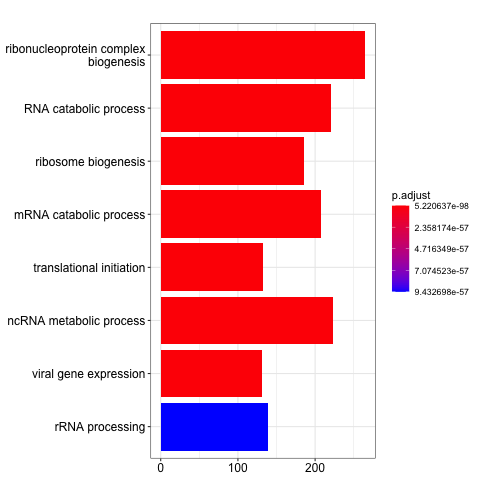
\includegraphics[scale = 0.3]{figures/barplotGenes2.png}
	\caption{Diagrama de las funciones m\'as importantes}
\end{figure}
\clearpage
